%Dokumentinnstillinger:---------------------------------
%Ved å google flitting kan du finne ut hva de forskjellige tingene her betyr, og hvordan du kan gjøre eventuelle endringer.
\documentclass[a4paper,11pt,norsk]{article}
\usepackage[utf8]{inputenc}
\usepackage{a4wide}
\usepackage{lmodern}
\usepackage[T1]{fontenc}
\usepackage{babel}

\setlength{\parindent}{0pt} 
\setlength{\parskip}{2ex}
\usepackage{fixltx2e}
\usepackage{amsmath}
\usepackage[pdftex, pdfborderstyle={/S/U/W 0}]{hyperref}
\usepackage{graphicx}
\usepackage[font=small,labelfont=bf]{caption}
\usepackage{tabularx}
\usepackage{multirow}
\usepackage{circuitikz}
\usepackage{pst-node,pst-circ}
% Adds seperation between two elements with a comma. Format: "    ,    ".
\newcommand{\comma}{\quad , \quad}
% Gives double underline under selected text.
\def\dunderline#1{\underline{\underline{#1}}}
% Faster way to make an equation that can be formatted with "&" to look nice.
\def\spliteq#1{\begin{equation}\begin{split}{#1}\end{split}\end{equation}\\}
%------------------------------------- End -------------------------------------

\begin{document}

%Headingdel:---------------------------------------------
\begin{minipage}[c]{0.15\textwidth}

\includegraphics[width=2.0cm]{elsys_pos_staaende_ntnu.png}
\end{minipage}
\begin{minipage}[c]{0.85\textwidth}

\renewcommand{\arraystretch}{1.7}
\large 
\begin{tabularx}{\textwidth}{|X|X|}
\hline
\multicolumn{2}{|l|}{} \\
\multicolumn{2}{|l|}{\huge \textbf{Designnotat 7}} \\
\multicolumn{2}{|l|}{}  \\
\hline
\multicolumn{2}{|l|}{Tittel: 
%Skriv inn tittel her:------------------------------------------
Anti-Aliasing Filter
} \\
\hline
\multicolumn{2}{|l|}{Forfattere: 
%Skriv inn forfattere her:--------------------------------------
Sindre Danielsen
} \\
\hline
%Skriv inn versjon og dato her her:-----------------------------
Versjon: 1.4 & Dato: 11.12.21
\\
\hline 
\end{tabularx}
\end{minipage}
\normalsize

%Automatisk generert innholdsfortegnelse:------------------

\setlength{\parskip}{0ex}
\renewcommand{\baselinestretch}{0.1}\normalsize
\tableofcontents
\renewcommand{\baselinestretch}{1.00}\normalsize
\setlength{\parskip}{2ex}
\rule{\textwidth}{1pt}

%Selve rapporten:----------------------------------------÷
\newpage
\section{Problembeskrivelse}
\label{sec: innledning}
Når et analogt signal skal filtreres, så brukes vanligvis digital signalbehandling. For å unngå at ADC omformeren skal få alvorlige \emph{aliasing-feil}, så burde båndbredden $B$ begrenses. Dette kan gjøres ved et \emph{anti-aliasing filter} slik vist i figur~\ref{fig: generell AAF}.
\\
\begin{figure}[htbp]
    \centering
    \begin{circuitikz} [american voltages, european resistors, baseline=(current bounding box.center)]
        \ctikzset { label/align = straight }
        \draw (0,0)
        node[draw,solid,minimum width=2.5cm,minimum height=2cm,anchor=south west] at (0,0) {Signalkilde}
    
        node[draw,solid,minimum width=4cm,minimum height=2cm,anchor=south west] at (4.5,0) {Anti-aliasing filter}
        
        node[draw,solid,minimum width=2cm,minimum height=2cm,anchor=south west] at (10.5,0) {ADC}
        
        node[] at (3.5, 1.5) {$v_1(t)$}
        node[] at (9.5, 1.5) {$v_2(t)$}
        ;
        \draw [-Triangle] (2.5,1) -- ++ (2,0);
        \draw [-Triangle] (8.5,1) -- ++ (2,0);
        
    \end{circuitikz}
    \caption{Filtrerer vekk uønskede frekvenser på signalet $v_1(t)$, som gir  signalet $v_2(t)$. }
  \label{fig: generell AAF}
\end{figure}
\\
Anti-alias filtreringen skal brukes ved en punktprøvingsfrekvens $f_s$, som er gitt ved $f_s = 2B$. En fullstendig båndbegrensning er derimot ikke mulig i praksis. Det er heller ikke nødvendig, så lenge frekvensene større enn $B$ blir svekket betydelig og frekvensene innenfor $B$ ikke blir vesentlig påvirket. Ved bruk av analoge filter, så er det mulig å oppnå ved en knekkfrekvens $f_c$ slik ønskelig.
\\\\
Krav til $v_2(t)$:
\begin{itemize}
    \item Dempning $A_{min} \leq -10$db ved $B$.
    \item Knekkfrevkensen ($-3$db fra maksimum amplituderespons.): \\
\begin{equation} \label{eq: f_c}
    f_c \geq 0.75 \frac{f_s}{2}
\end{equation}
\end{itemize}





\newpage
\section{Prinsipiell løsning}
\label{sec:prinsipielllosning}
Et anti-aliasing filter kan utvikles ved bruk av et lavpass filter. Enten det er bruk av RC filter, RCL filter eller andre muligheter som Butterworth- eller Chebeschev filter. Merk at spolen i et RCL filter vil i virkeligheten ha litt motstand, spesielt for større spoler. \\
\\
Et aktivt lavpass filter, som holder passbandet maksimalt flatt, samt en valgbar dempning ved $B$ er Butterworth filteret. Det har flatere knekkfrekvens enn Chebeschev filter, men til gjengjeld, så er det neglisjerbare forstyrrelser for amplituderesponen i og utenfor $B$. Filter design på analoge signal går ut ifra et system som er sensitivt for forstyrrelse i amplituderesponsen og derfor velges et Butterworth filter, slik vist i figur~\ref{fig: aktivt lavpass-filter}.
\begin{figure}[htbp]
	\centering
	\begin{circuitikz}
		\draw
		(0,0) node[op amp,yscale=-1](opamp){}

		(opamp.+) 	to [short] 					++(-1,0) 			coordinate(C2)
					to [C, l_=$C_2$, *-] 		++(0,-2)
					to ++(0,0) 										node[ground]{}

		(C2) 		to [R, l_=$R$] 				++(-2,0) 			coordinate(R2)
					to [short, *-] 				++(0,1) 			coordinate(C1)
					to [C, l=$C_1 $] 			(C1-|opamp.out) 
					to [short, -*] 				(opamp.out)

		(R2) 		to [R, l_=$R$, -o] 			++(-2,0) 			node[left] {$v_1(t)$}

		(opamp.-) 	to [short] 					++(0,-1) 			coordinate(fb)
					to [short] 					(fb-|opamp.out) 
					to [short] 					(opamp.out)
					to [short, -o] 				++(1,0) 			node[right] {$v_2(t)$}

		;
	\end{circuitikz}
	\caption{2.ordens Butterworth filter med Sallen-Key kretstopologi \cite{Sallen-Key topology}.}
	\label{fig: aktivt lavpass-filter}
\end{figure} \\
Filteret filtrerer ut de høye frekvensene fra $v_1(t)$ og sender ut et signal $v_2(t)$ som har de lave frekvensene påtrykket.
Det er vanlig at motstandene $R$ i kretsen er like hverandre, som gjør analysen lettere. Dersom et 1. ordens filter ønskes, så kan kondensatoren $C_1$ fjernes. Kondensatoren $C_2$ i samband med $C_1$ skaper et 2. ordens filter.
\\\\
For å utvikle filteret som nevnes i seksjon~\ref{sec: innledning}, så er likningen for et Butterworth filter gitt ved:
\begin{equation} \label{eq: butterworth}
    A_{min} = |H(j2\pi)| = \frac{1}{\sqrt{1+ \left(\frac{f_c}{B}\right)^{2n}}},
\end{equation}
Den generelle formelen har en $\epsilon^2$ fremfor $\left(\frac{f_c}{B}\right)^{2n}$, men vanligvis er $f_c = -3$db$ \implies \epsilon^2 = 1$. For mer informasjon om Butterworth filter, se \cite{Butterworth-filter}.
\newpage
N-orden gir informasjon om hvor mange poler som eksisterer:
\begin{itemize}\label{list: filter}
    \item $n=1 \implies$ 1. ordens lavpass filter.
    \item $n=2 \implies$ 2. ordens lavpass filter
    \item $n > 2 \implies$  1. ordens- og 2. ordens-lavpass filter i seriekopling.
\end{itemize}
Det er derfor essensielt å finne n-orden på kretsen, som kan gjøres ved å omforme likning~\ref{eq: butterworth} til
\begin{equation}\label{eq: n-orden}
    n = \frac{1}{2} \frac{ln(A^{-2}-1)}{ln\left( \frac{f_c}{B} \right)}.
\end{equation}
Merk at $n$ skal være et heltall. Ved desimaler, så rundes $n$ opp til neste heltall. Å runde ned $n$ impliserer at $A_{min}$ vil øke. Da er det heller bedre å oppnå en større dempning enn ønsket ved å øke $n$. Ønskelig frekvensspekter av $v_2(t)$ for et Butterworth filter er vist ved det begrensede området i figur~\ref{fig: Butterworth signal}.
\\
\begin{figure}[htbp]
    \centering
    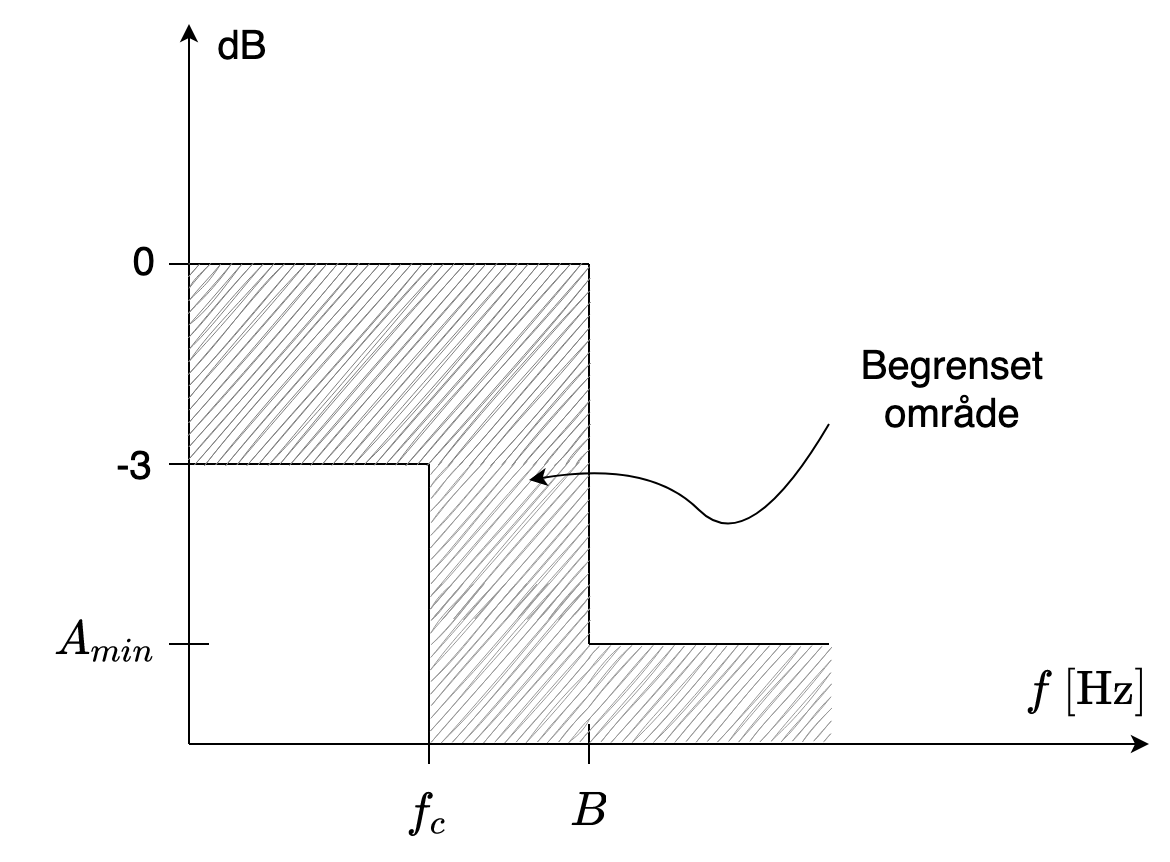
\includegraphics[width=1.0\textwidth]{img/Skisse signal.PNG}
    \caption{Frekvensresponsen til et Butterworth filter.}
    \label{fig: Butterworth signal}
\end{figure} \\
\newpage
Filteret vil ha tidskonstantene gitt ved
\begin{equation}\label{eq: tidskonstant}
    \tau_1 = \frac{1}{2\pi f_c \zeta} \quad , \quad \tau_2 = \frac{1}{(2\pi f_c)^2 \tau_1} \: .
\end{equation}
Et 1. ordens system vil kun ta i bruk $\tau_1$. \\\\
Kondensatorene er gitt ved 
\begin{equation} \label{eq: kondensator}
    C_1 = \frac{\tau_1}{R} \quad , \quad C_2 = \frac{\tau_2}{R} \: .
\end{equation}
Vi mangler dempningsfaktoren $\zeta$. Den kan eventuelt finnes grafisk ved å dele opp en  halvsirkel for en reell- (x-aksen) og imagineær-akse (y-aksen). Det første komplekskonjugerte polparet $n = 2$ plasseres $\pm 45^{\circ}$. Hvis $n = 4$, så plasseres to komplekskonjugerte polpar på $\pm \left(45^{\circ} + \frac{45^{\circ}}{2}\right)$ og $\pm\left(45^{\circ} - \frac{45^{\circ}}{2}\right)$. Slik kan man fortsette for høyere N-orden. Det er vanlig å lese av $\zeta$ for den reelle verdien. Dette kan være tungvint å gjenta seg, så legger ved en liste for $n\in[1, 10]$, som vist ved tabell~\ref{table: N-orden}. Merk at alle verdier $\zeta_{1},\: \zeta_{1},\:... \:\: \zeta_{n}$ har samme $f_c$, siden systemet er lineært innenfor opampens virkeområde. 
\newpage
\begin{table}[htbp]
\centering
\begin{tabular}{ |c|c|c|c| } 
\hline
\textbf{N-Orden $n$} & \textbf{Reelle Verdier $\zeta$} & \textbf{N-Orden $n$} & \textbf{Reelle Verdier $\zeta$} \\
\hline
1 & $1.0000$ & 6 & $0.9659$ \\
&&& $0.7071$ \\
&&& $0.2588$
\\
\hline
2 & $0.7071$ & 7 & $0.9010$ \\
&&& $0.6235$ \\
&&& $0.2225$ \\
&&& $1.0000$
\\
\hline
3 & $0.5000$ & 8 & $0.9808$ \\
& $1.0000$ && $0.8315$ \\
&&& $0.5556$ \\
&&& $0.1951$
\\
\hline
4 & $0.9239$ & 9 & $0.9397$ \\
&$0.3827$& & $0.7660$ \\
& & & $0.5000$ \\
&&&$0.1737$ \\
&&&$1.0000$
\\
\hline
5 & $0.8090$ & 10 & $0.9877$ \\
& $0.3090$ & & $0.8910$\\
& $1.1000$ & & $0.7071$\\
& & & $0.4540$\\
& & & $0.1564$
\\
\hline
\end{tabular}
\caption{Butterworth pol lokasjoner for $\zeta$ av $n\in[1, 10]$}
\label{table: N-orden}
\end{table}
\\
En notasjon ved bruk av opamper er å velge $R\in[1\textrm{k}\Omega, 100\textrm{k}\Omega]$. Årsaken er at i dette området vil kretsen trekke minst mulig strøm og ha en neglisjerbar følsomhet for støy når det kommer til opamper. Det kalles \textit{opampens gyldne regel}.

\\\\ Generelt sett er det en enkel metodikk for utvikling av Butterworth filter: 
\begin{enumerate}
    \item Velg en $R$ innenfor området gitt av den gylne regel for opamper. 
    \item Regn ut N-orden for å finne antall butterworth-filter.
    \item Finn $\zeta$ verdiene.
    \item Regn ut kondensatorverdiene.
\end{enumerate}


\newpage
\section{Realisering og test}
\label{sec:realisering}
Oppkoblingen av kretsen bruker komponentverdiene gitt ved tabell~\ref{table: reelle verdier}.
\begin{table}[htbp]
\centering
\begin{tabular}{ |c|c|c|c| } 
\hline
\textbf{Navn} & \textbf{Verdi} & \textbf{Beskrivelse}\\
\hline
opamp & LF353N & Tilgjengelige opamper.
\\
\hline
$R$ & $1$k$\Omega$ & Valgt motstand (innenfor opampens gyldne regel).
\\
\hline
$C_{1, 1}$ & $172$nF & 1. Kondensator for 1. filter (likning~\ref{eq: kondensator}). 
\\
\hline
$C_{1, 2}$ & $147$nF & 2. Kondensator for 1. filter.
\\
\hline
$C_{2, 1}$ & $416$nF & 1. Kondensator for 2. filter.
\\
\hline
$C_{2, 2}$ & $60.9$nF & 2. Kondensator for 2. filter.
\\
\hline
\end{tabular}
\caption{Reelle verdier basert på tabell~\ref{table: teoretiske verdier}}
\label{table: reelle verdier}
\end{table}
\\
\begin{table}[htbp]
\centering
\begin{tabular}{ |c|c|c|c| } 
\hline
\textbf{Navn} & \textbf{Verdi} & \textbf{Beskrivelse}\\
\hline
$f_s$ & $7.6$kHz & Valgt samplingsfrekvens. \\
\hline
$B$ & $3.8$kHz & Gitt ved $f_s / 2$. \\
\hline
$f_c$ & $\geq 2.85$kHz & Knekkfrekvens ved $\geq 0.75 B$. \\
\hline
$A_{min}$ & $-10$dB & Ønsket dempning ved $B$.
\\
\hline
$n$ & $4$ & N-orden fra likning~\ref{eq: n-orden}.
\\
\hline
$\tau_{1, 1}$ & $60.4\mu$s & 1. tidskonstant for 1. filter (likning~\ref{eq: tidskonstant}).
\\
\hline
$\tau_{1, 2}$ & $51.6\mu$s & 2. tidskonstant for 1. filter.
\\
\hline
$\tau_{2, 1}$ & $145.9\mu$s & 1. tidskonstant for 2. filter.
\\
\hline
$\tau_{2, 2}$ & $21.4\mu$s & 2. tidskonstant for 2. filter.
\\
\hline
$R$ & $1$k$\Omega$ & Valgt motstand (innenfor opampens gyldne regel).
\\
\hline
$C_{1, 1}$ & $60.4$nF & 1. Kondensator for 1. filter (likning~\ref{eq: kondensator}). 
\\
\hline
$C_{1, 2}$ & $51.6$nF & 2. Kondensator for 1. filter.
\\
\hline

$C_{2, 1}$ & $145.9$nF & 1. Kondensator for 2. filter.
\\
\hline
$C_{2, 2}$ & $21.4$nF & 2. Kondensator for 2. filter. 
\\
\hline
\end{tabular}
\caption{De teoretiske verdiene av komponentene i figur~\ref{fig: n = 4 Butterworth filter}. }
\label{table: teoretiske verdier}
\end{table}
\\
\newpage
Endrer figur~\ref{fig: aktivt lavpass-filter} for $n = 4$, som vist ved figur~\ref{fig: n = 4 Butterworth filter}. \\
\begin{figure}[htbp]
	\centering
	\begin{circuitikz}
		\draw
		(0,0) node[op amp,yscale=-1](opamp){}

		(opamp.+) 	to [short] 					++(-1,0) 			coordinate(C2)
					to [C, l_=$C_{1, 2}$, *-] 		++(0,-2)
					to ++(0,0) 										node[ground]{}

		(C2) 		to [R, l_=$R$] 				++(-2,0) 			coordinate(R2)
					to [short, *-] 				++(0,1) 			coordinate(C1)
					to [C, l=$C_{1, 1}$] 			(C1-|opamp.out) 
					to [short, -*] 				(opamp.out)

		(R2) 		to [R, l_=$R$, -o] 			++(-2.3,0) 			node[left] {$v_1$}

		(opamp.-) 	to [short] 					++(0,-1) 			coordinate(fb)
					to [short] 					(fb-|opamp.out) 
					to [short] 					(opamp.out)
					to [short] 				++(0.4,0)

		;
		\draw
		(7.8,0) node[op amp,yscale=-1](opamp){}

		(opamp.+) 	to [short] 					++(-1,0) 			coordinate(C2)
					to [C, l_=$C_{2, 2}$, *-] 		++(0,-2)
					to ++(0,0) 										node[ground]{}

		(C2) 		to [R, l_=$R$] 				++(-2,0) 			coordinate(R2)
					to [short, *-] 				++(0,1) 			coordinate(C1)
					to [C, l=$C_{2, 1}$] 			(C1-|opamp.out) 
					to [short, -*] 				(opamp.out)

		(R2) 		to [R, l_=$R$] 			++(-2,0) 
		--                                      ++ (0, -0.5)

		(opamp.-) 	to [short] 					++(0,-1) 			coordinate(fb)
					to [short] 					(fb-|opamp.out) 
					to [short] 					(opamp.out)
					to [short, -o] 				++(1,0) 			node[right] {$v_2$}
		;
		\draw
        node[label=2. ordens Butterworth filter nr. 1,
        draw,dashed,minimum width=7.50cm,minimum height=6cm,anchor=south west
        ] 
        at (-6.1,-2.5) {}
		;
		\draw
        node[label=2. ordens Butterworth filter nr. 2,
        draw,dashed,minimum width=7.50cm,minimum height=6cm,anchor=south west
        ] 
        at (-6.1+7.9,-2.5) {}
		;
	\end{circuitikz}
	\caption{Anti-aliasing filter: 4. ordens Butterworth filter.}
	\label{fig: n = 4 Butterworth filter}
\end{figure} \\
Verdiene på $\tau$ utreknes ved bruk av $n = 4$ i tabell~\ref{table: N-orden}, der $\zeta_1 = 0.9239$ for første filteret og $\zeta_2 = 0.3827$ for det andre.


Siden kondensatorverdiene og $R$ er ulike fra tabell~\ref{table: teoretiske verdier} til tabell~\ref{table: reelle verdier}, så kan det være lurt å rekne ut frekvensene $B$ og $f_c$ for de nye verdiene. Vi kan da få få en idé om det forventede resultatet ved frekvensanalysen.
Isolering av $f_c$ i likning~\ref{eq: tidskonstant} for $\tau_2$ gir at 
\begin{equation} \label{eq: f_c likning}
    f^*_c = \frac{\zeta_1}{2\pi R C_{12}} = 2905.0 \textrm{Hz}.
\end{equation}
Merk at kondensatorer har toleranseområde på kapitansen, som varierer på komponentene, så det kan gi minimale avvik i resultatet.\\\\
Forventer å få $A_{min} = -10$dB ved
\begin{equation}\label{eq: Båndbredde}
    B^* = \frac{f_c}{0.75} = 3873.4\textrm{Hz}.
\end{equation}
\newpage
Kobler opp kretsen som vist i figur~\ref{fig: realKrets} og sammenlikner tidligere utrekninger med figur~\ref{fig: frekvensspekter}.
\begin{figure}[htbp]
    \centering
    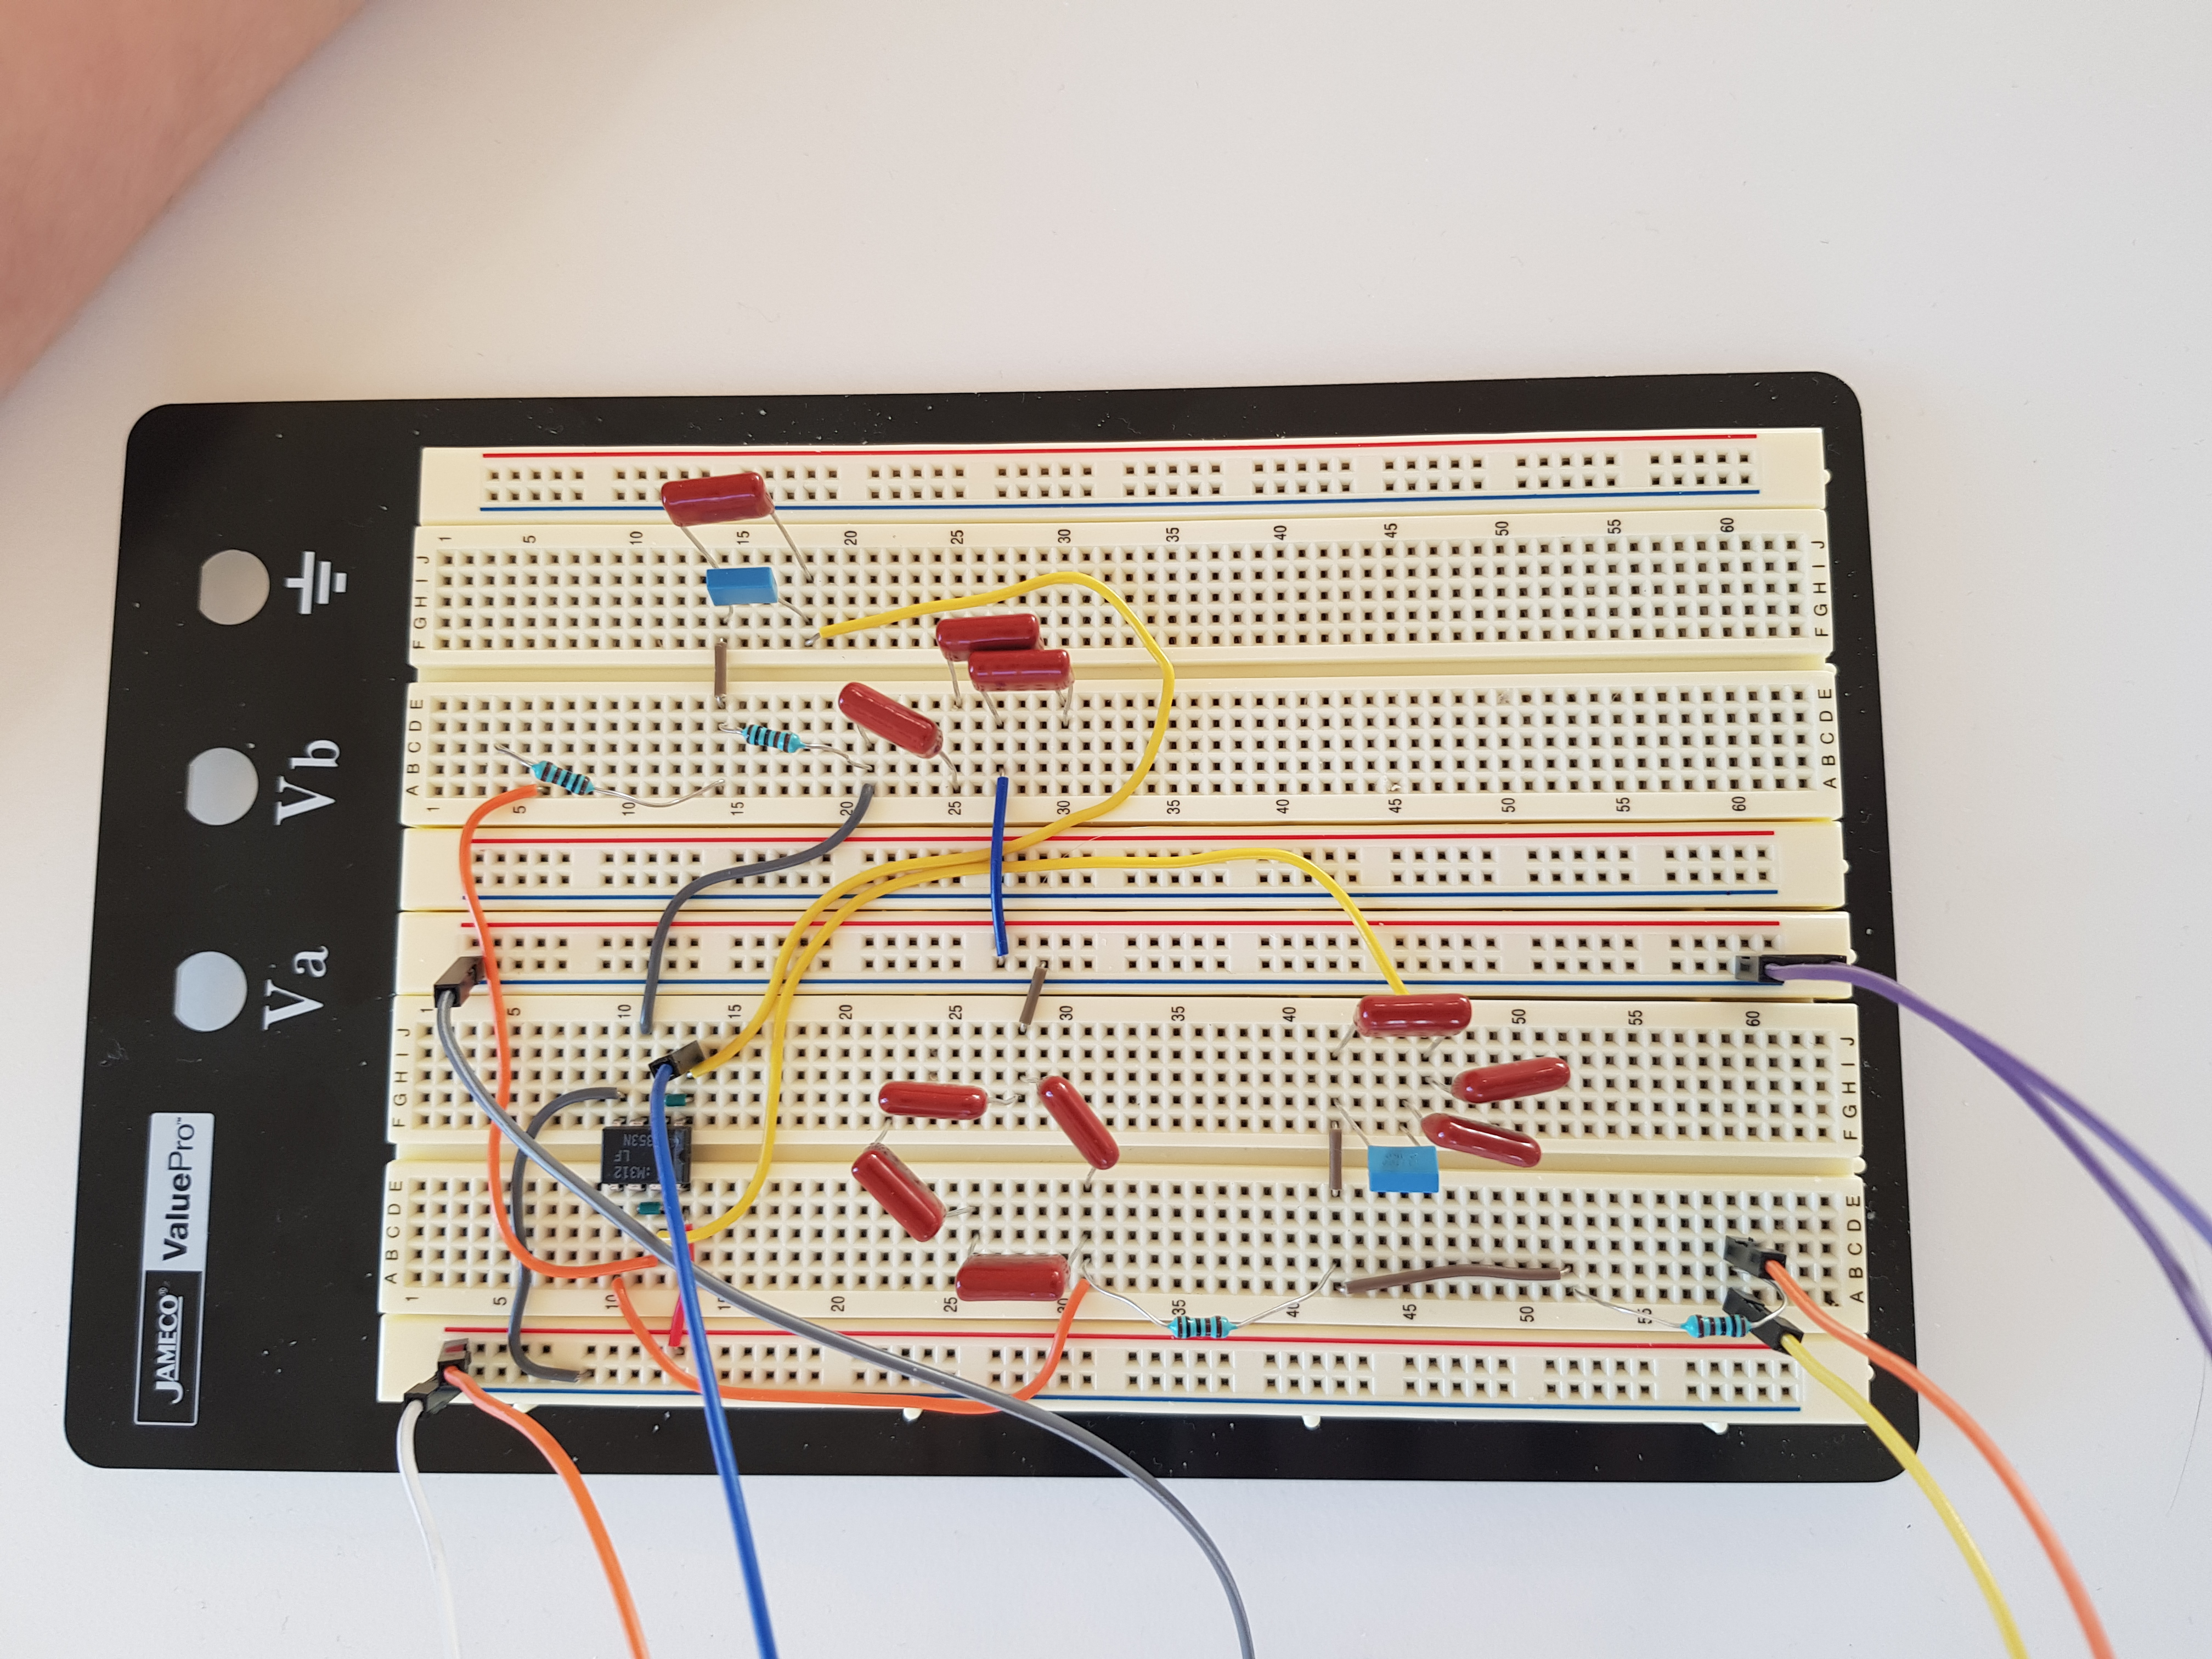
\includegraphics[width = 1.0 \textwidth]{img/RealKretsDp7.jpg}
    \caption{Realiseringen av figur~\ref{fig: n = 4 Butterworth filter}.}
    \label{fig: realKrets}
\end{figure} \\


\begin{figure}[!htbp]
    \centering
    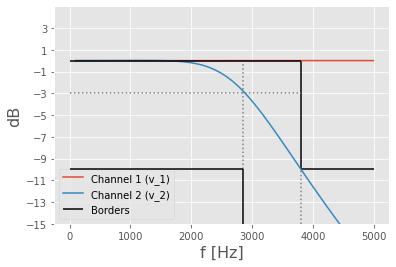
\includegraphics{img/Butterworth.png}
    \caption{Frekvensspekter av figur~\ref{fig: n = 4 Butterworth filter} med grensene (borders) fra figur~\ref{fig: Butterworth signal}.}
    \label{fig: frekvensspekter}
\end{figure} \\
\newpage
Fra figur~\ref{fig: frekvensspekter} kan vi ved å observere nøye, se at amplituderesponsen til $v_2(t)$ ligger innenfor ønsket området for et Butterworth filter. Merk at der de stiplede linjene krysser hverandre gir en mindre frekvens enn der den horisontale stiplede linjen på $-3dB$ krysser $v_2(t)$. Det betyr at kravet om $f_c \geq 2.85$kHz er verifisert. For mer nøyaktige verdier, så kan det brukes markører (cursors) i oscilloskop. Verdiene for $f_c$, $f_c^*$, $B$ og $B^*$ er vist i figur~\ref{fig: markører}.
\begin{figure}[!htbp]
    \centering
    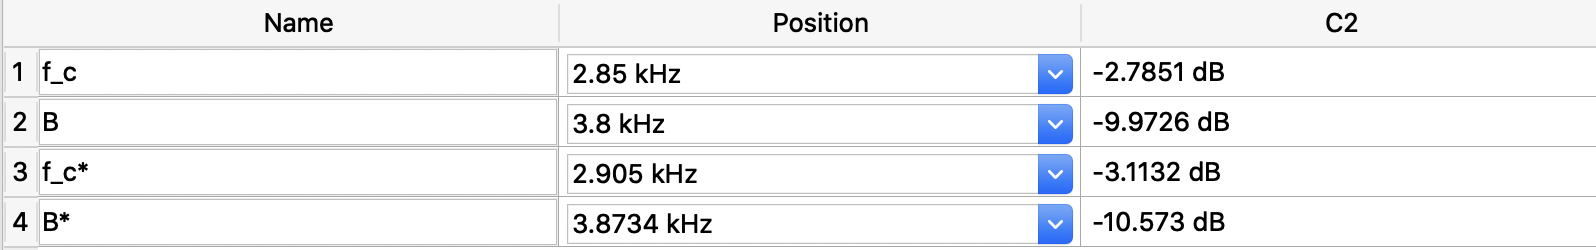
\includegraphics[width = 1.0 \textwidth]{img/Cursors_main.png}
    \caption{Markører for $f_c$ og $B$.}
    \label{fig: markører}
\end{figure}\\

Verdiene for $C2$ gir at kravene satt i seksjon~\ref{sec: innledning} ikke overholdes for $A_{min}$ eller $f_c$, dersom det brukes $f_c^*$ og $B^*$. \newpage
\section{Konklusjon}
\label{sec:konklusjon}
For utvikling av et anti-aliasing filter ved bruk av Butterworth filter design, så kreves det nøyaktighet i komponentverdier, herunder kondensatorer og motstander.. I tillegg kan det også kreve flere lavpass filter for å oppnå ønskelig $A_{min}$. Flere kaskadekoblede Butterworth filter gir en brattere knekkfrekvens. Butterworth filter med Sallen-Key topologi oppnår oppførselen vi et ute etter dersom kondensatorverdiene og motstandene overholder likningene beskrevet i seksjon~\ref{sec:prinsipielllosning}.
De teoeretisk ønskede verdiene for $f_c$ og $B$ overholder kravene satt i seksjon~\ref{sec: innledning}. 
\newpage

\begin{thebibliography}{9}
\bibitem{Butterworth-filter}
    ElectronicsTutorials. (Ukjent), Article \\
    \emph{Butterworth Filter Design} \\
    Tilgjengelig ved: \href{https://www.electronics-tutorials.ws/filter/filter_8.html}{https://www.electronics-tutorials.ws/filter/filter_8.html} \\
    (Sist åpnet: 7. November 2021)

\bibitem{Sallen-Key topology}
    ElectronicsTutorials (2021),  \\
    \emph{Sallen and Key Filter} \\
    Tilgjengelig ved: \\
    \href{https://www.electronics-tutorials.ws/filter/sallen-key-filter.html}{https://www.electronics-tutorials.ws/filter/sallen-key-filter.html} \\
    (Sist åpnet: 7. November 2021) 
\end{thebibliography}
\newpage
%Bibliografi: Legg til flere elementer ved å legge til flere \bibitem:--------
\phantomsection

\appendix
%Tillegg. Flere tillegg legges til ved å lage flere sections:-----------------


\end{document}